\chapter{Introduction}

\denis

Versatile Object-oriented Toolkit for Coarse-graining Applications, or \votca, is a package which helps to systematically coarse-grain various systems. This includes  deriving the coarse-grained potentials, assessing their quality, preparing input files required for coarse-grained simulations, and analysing the latter. 

A typical coarse-graining workflow includes {\em sampling} of the system of interest, {\em analysis} of the trajectory using a specific {\em mapping scheme} and a coarse-graining {\em method} to derive coarse-grained potentials and, in case of iterative methods, running coarse-grained simulations and iteratively {\em refining} the coarse-grained potentials.

The workflow can be exemplified on coarse-graining of a propane liquid. A single molecule of propane contains three carbon and eight hydrogen atoms. A united atom coarse-grained representation of a propane molecule has three beads and two bead types, A and B, with three and two hydrogens combined with the corresponding atom, as shown in \fig{fig:intro:propane}. This representaion defines the \hyperref[sec:mapping_operator]{mapping operator}, as well as the bonded corse-grained degrees of freedom, such as the bond $b$ and the bond angle $\theta$. The task of coarse-graining is then to derive a potential energy surface which is a function of these coarse-grained degrees of freedom.

\begin{wrapfigure}{r}{4cm}
 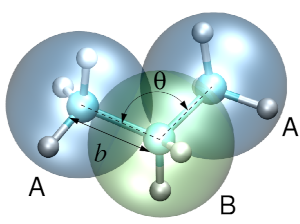
\includegraphics[width=4cm]{fig/propane}
 \caption{\small Three-bead coarse-grained model of propane.
 \label{fig:intro:propane}
}
\end{wrapfigure}

While the atomistic bond and angle potentials are often chosen to be simple harmonic functions, the coarse-grained potentials cannot be expressed in terms of simple analytic functions. Instead, tabulated representations are normally used. 

The coarse-graining {\em method} defines criteria according to which the potential energy surface is constructed. For example, {\em Boltzmann Inversion} provides us with a potential of mean force. {\em Iterative Boltzmann Inversion} and {\em Inverse Monte Carlo} methods aim at reproducing radial distribution functions. {\em Force Matching} (or multiscale coarse-graining) approximates the many-body potential of mean force.

In most cases, coarse-graining requires canonical sampling of a reference (high resolution) system. In addition, iterative methods require canonical sampling of the coarse-grained system. The sampling can be done using either molecular dynamics (MD), stochastic dynamics (SD), or Monte Carlo (MC) techniques. The latter are implemented in many standard simulation packages. Rather than implementing its own MD/SD/MC modules, \votca allows swift and flexible integration of existing  programs in such a way that sampling is performed in the program of choice. The analysis needed for systematic coarse-graining is done using the package tools.

More details as well as several examples can be found in~\ref{Ruehle:2009.a}. 